\Chapter{Koncepció}

% Ez a fejezet még nem a saját eredményekkel foglalkozik, hanem bemutatja, mi a problémakör, milyen módszerekkel, milyeneredményeket sikerült elérni eddig másoknak.

% A hivatkozások jelentős része ehhez a fejezethez szokott kötődni.
% (Egy hivatkozás például így néz ki \cite{coombs1987markup}.)
% Itt lehet bemutatni a hasonló alkalmazásokat.

% A fejezet tartalma témától függően változhat. Az alábbiakat attól függően különböző arányban tartalmazhatják.

% % Amit csak említés szintjén érdemes szerepeltetni

% Az olvasóról annyit feltételezhetünk, hogy programozásban valamilyen szinten járatos, és a matematikai alapfogalmakkal sem ebben a dolgozatban kell megismertetni.
% A speciális eszközök, programozási nyelvek, matematikai módszerekk és jelölések persze jó, hogy ha említésre kerülnek, de nem kell nagyon belemenni a közismertnek tekinthető dolgokba.

\Section{Irodalomkutatás}

% Amennyiben a dolgozat egy módszer kidolgozására, kifejlesztésére irányul, akkor itt lehet részletesen végignézni (módszertani vagy időrendi bontásban), hogy az eddigiekben milyen eredmények születtek a témakörben.

\SubSection{Egységtesztelés}

Az egységtesztelés (unit testing) a szoftvertesztelés egy olyan módszere, amely során a forráskód legalacsonyabb szintű, a programot felépítő egységeket tesztelik. A szoftvertesztelés szintjei \aref{fig:software_testing_levels}. ábrán látható. Az egység egy rendszer legkisebb önálló egységként tesztelhető része. Az egységtesztekkel ellenőrizhető, hogy egy egység az elvárásoknak megfelelően működik. Egy egység függvényeiről ellenőrizzük, hogy különböző bemenetek esetén megfelelő eredményt, vagy hibát produkálnak. Az egységeket egymástól függetlenítve kell tesztelni.

\begin{figure}[h]
    \centering
    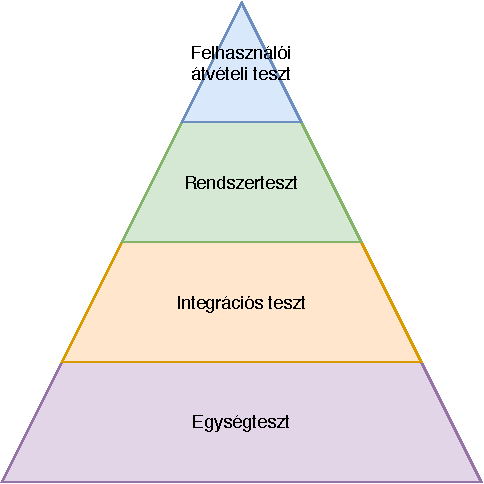
\includegraphics{images/software_testing_levels.pdf}
    \caption{A szoftvertesztelés szintjei.}
    \label{fig:software_testing_levels}
\end{figure}

Az egységtesztelés nem egy új fogalom a szoftverfejlesztésben. Az 1970-es évektől, a Smalltalk programozási nyelv korai napjai óta jelen van, és ez az egyik legjobb módszer arra, hogy a fejlesztő növelje a kód minőségét miközben jobban megérti az adott osztály vagy metódus működését. Kent Beck amerikai szoftvermérnök vezette be az egységtesztelés koncepcióját, majd ezután az egységtesztelés, mint fogalom átöröklődött sok más programozási nyelvbe is, ezzel az egységtesztelést egy rendkívül hasznos, és nyelvfüggetlen gyakorlattá téve. \cite{osherove_2013_the-art-of-unit-testing}

Beck az egységtesztelést a Smalltalk nevű programozási nyelvben implementálta az SUnit egységtesztelő keretrendszerként \cite{beck_1999_guide-to-better-smalltalk}. Ezután a keretrendszert a fejlesztői közösség adaptálta más programozási nyelvekre is és megtartották a Beck által bevezetett terveket, ötleteket. Az SUnit-ot alapul vevő egységtesztelő keretrendszereket nevezzük összefoglaló néven xUnit keretrendszereknek. \cite{fowler_2006_xunit}

Napjainkban a legnépszerűbb egységteszt keretrendszerek mind az xUnit keretrendszercsaládba tartoznak.

\SubSection{Tesztvezérelt fejlesztés}

A tesztvezérelt fejlesztés (Test-driven Development, TDD) napjaink egyik legismertebb szoftverfejlesztési folyamata a professzionális programozásban. Ez a folyamat nagyon rövid fejlesztési ciklusokon alapul: a követelmények nagyon specifikus tesztesetekként vannak megfogalmazva, a kódot pedig ahhoz mérten írjuk, hogy az át fog így menni a teszten. Ez teljes ellentettje a hagyományos szoftverfejlesztésnek, mivel az megengedi azon kódrészleteket is, amelyek nem felelnek meg a követelményeknek teljesen.

Az egységteszteléshez hasonlóan ez is Kent Beck-től ered. Őt tartjuk számon a technika kifejlesztéséért, és újrafelfedezésért. Beck a tesztvezérelt fejlesztésről először egy régi programozásról szóló könyvben olvasott, majd amikor megírta az első xUnit keretrendszert a Smalltalk nyelvben, akkor emlékezett erre, majd kipróbálta ezt saját maga is. \cite{beck_2012_tdd-rediscovery} A tesztvezérelt fejlesztés folyamatát az extrém programozás (Extreme Programming, XP) nevű módszertan részeként tökéletesítette és ekkor vált népszerűvé ez a módszer a programozók körében.

\begin{figure}[h]
    \centering
    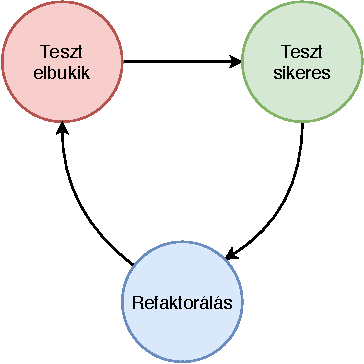
\includegraphics{images/tdd_steps.pdf}
    \caption{A tesztvezérelt fejlesztés ciklusa és azon lépései.}
    \label{fig:tdd_steps}
\end{figure}

A tesztvezérelt fejlesztés ciklusának \aref{fig:tdd_steps} ábrán látható lépései kifejtve: \cite{beck_2003_tdd}
\begin{enumerate}
    \item \textbf{Tesztírás}

          Minden új funkció fejlesztése tesztek írásával kezdődik. Minden frissíteni kívánt vagy újdonsült metódushoz írjunk egy tesztet ami röviden és tömören lefedi az új funkciót. Ehhez a fejlesztőnek tisztán értenie kell a funkció specifikációját és követelményeit. A fejlesztő ezt használati eset (use case) diagramokon vagy felhasználói történeteken (user story) keresztül értheti meg a követelményeket, majd ezek után foghat neki megírni a teszteseteket. Ezek lehetnek már meglévő tesztesetek bővítései is, ha egy meglévő funkciót bővít ki.

    \item \textbf{Tesztfuttatás}

          A tesztesetek megírása után mindenképpen érdemes lefuttatni azokat, mivel jelen állapotban minden tesztesetnek el kell buknia. Ilyenkor még nincs az új funkcióhoz tartozó programkód megírva, és az ilyenkor elbukott tesztesetek garantálják azt, hogy nem írt a programozó olyan tesztet ami mindig sikeres, ami hibás lenne.

    \item \textbf{Kódírás}

          Ebben a lépésben a fejlesztő megírja a tesztesetekhez tartozó működő programkódot. Fontos, hogy az itt megírt programkódnak nem kell tökéletesnek lennie, itt az a cél, hogy mindegyik teszteset sikeresen lefusson. A programozónak nem szabad a teszteseteket meghaladó, a specifikáción és követelményeken kívül eső kódot írnia.

    \item \textbf{Tesztfuttatás}

          Ha az összes teszteset sikeresen lefut, akkor a programozó biztos lehet benne, hogy az új kód megfelel a teszt specifikációknak és nem tör el vagy ront el más funkciókat. Ha a tesztesetek közül legalább 1 darab nem fut le, akkor a kódot addig kell javítanunk míg az összes teszteset sikeres nem lesz.

    \item \textbf{Refaktorálás}

          A növekvő kódbázist folyamatosan takarítani kell a tesztvezérelt fejlesztés során. Az új kód átmozgatásra kerülhet a logikailag, és strukturálisan megfelelő helyére. A kódduplikációkat ki kell szervezni, el kell távolítani. A osztályaink, változóink és metódusaink elnevezését javítani kell, hogy mások is tisztán érthessék a funkciókat. Ahogy új és új funkciók hozzáadásra kerülnek az osztályaink és a metódusaink egyre és egyre hosszabbak lesznek, ezeket gondosan szét kell darabolni több részre az olvashatóság és karbantarthatóság miatt.

          A tesztesetek folyamatos futtatása segíti abban a fejlesztőt, hogy a refaktorálás lépése alatt elvégzett kód átírások során nem tör el semmi funkciót és a tesztek ugyanúgy sikeresen lefutnak.
\end{enumerate}

\SubSection{Egységtesztelés a C\# programozási nyelvben}

A C\# programozási nyelvben nincs gyári, beépített (azaz a .NET keretrendszerrel érkező) egységtesztelő keretrendszer, így mind a tesztek írásához, futtatásához és az eredmények megjelenítéséhez szükségünk van egy ezt támogató bővítményre.

Napjainkban a legnépszerűbb egységteszt keretrendszerek a következők:
\begin{itemize}
    \item[--] Visual Studio Unit Testing Framework (,,MSTest'')
    \item[--] xUnit.net
    \item[--] NUnit
\end{itemize}

Mindhárom keretrendszer ingyenes, és nyílt forráskódú. Az MSTest keretrendszert habár a Microsoft fejleszti, szintén mint a C\# nyelvet és a .NET környezetet, de ez nincs a környezetbe integrálva. Az xUnit.net-et a Microsoft hivatalosan is használja több szoftverének tesztelésében is, például az ASP.NET Core forráskódhoz ezzel a keretrendszerrel készítik az egységteszteket.

A szakdolgozatban keretében a xUnit.net keretrendszer kerül felhasználásra.

Ezeket a keretrendszereket többféleképpen is elérhetjük a programunkban.
Legegyszerűbb módja ennek a keretrendszer bináris csomagjának a NuGet csomagkezelő rendszeren való letöltése, de ezenkívül a nyílt forráskódú csomagokat mi is lefordíthatjuk és manuálisan behivatkozhatjuk a projektfájlunkban, vagy akár a keretrendszer honlapjáról is letölthetjük a már lefordított binárisokat.

Miután telepítettük az általunk választott keretrendszert, elkezdhetünk írni egységteszteket a kódunkhoz. Minden megfelelően annotált metódus egy teszteset amiben egy másik adott kódot tesztelünk. Minden keretrendszernél kicsit másképpen néz ki a tesztek felépítése, de bevett szokás az, hogy az teszteseteket tartalmazó metódusokat annotálnunk kell. xUnit.net esetén a metódust a \texttt{Fact} ("mindig igaz" teszteset) vagy \texttt{Theory} ("a megfelelő adatra igaz" teszteset) attribútummal kell annotálnunk, ezzel jelezzük a keretrendszerünknek, hogy az adott metódus egy teszteset.

Nagyobb kódbázis esetén átláthatatlan ha minden tesztesetet a tesztelendő osztályba raknánk bele ezért más keretrendszereknél elvárt az, hogy az egységteszteink számára új osztályt hozzunk létre. Bevett szokás az, hogy új projektet hozunk létre ahol csak a tesztek osztályait és azok segítő osztályait tároljuk, de az is elegendő ha a meglévő projektben hozzuk létre az egységteszt osztályainkat. Az osztály létrehozása után, metódusonként írhatjuk meg a teszteseteinket. Az xUnit.net-nél erre nincs szükség, azonban javasolt, hogy elkülönítve és jól megnevezve tároljuk a teszteseteket tartalmazó osztályokat és magukat a metódusokat.

Minden keretrendszerben elérhető egy \texttt{Assert} osztály, amivel állításokat tehetünk a tesztjeinkbe. Ellenőrizhetjük, hogy például a metódusunk visszatérési értéke azaz az tényleges (actual) érték megegyezik-e a várt (expected) értékkel. Ezenkívül szinte bármilyen más feltételt ellenőrizhetünk. Például, hogy a tényleges érték tartalmaz-e valamit, üres-e, a várt típusú-e vagy, hogy éppen dob-e kivételt vagy sem. A teszteset akkor kerül sikeres (pass) állapotba, ha minden állításnak megfelelt, és közben nem dobott-e a programunk le nem kezelt kivételt. Ha ezeket nem teljesíti a tesztesetünk akkor sikertelen (fail) állapotba kerül.

\Section{Piackutatás}

% Bizonyos témáknál új termék vagy szolgáltatás kifejlesztése a cél.
% Ekkor érdemes annak alaposan utánanézni, hogy aktuálisan milyen eszközök érhetők el a piacon.
% Ez szoftverek esetében a hasonló alkalmazások bemutatását, táblázatos formában történő összehasonlítását jelentheti.
% Szerepelhetnek képek és észrevételek a viszonyításként bemutatott alkalmazásokhoz.

\Section{Követelmény specifikáció}

% Külön szakaszban érdemes részletesen kitérni az elkészítendő alkalmazással kapcsolatos követelményekre.
% Ehhez tartozhatnak forgatókönyvek (\textit{scenario}-k).
% A szemléletesség kedvéért lehet hozzájuk képernyőkép vázlatokat is készíteni, vagy a használati eseteket más módon szemléltetni.
